% \newgeometry{top=4cm,left=4cm,right=4cm,bottom=4cm} 
%
\section{Introduction}
It is hardly a controversial statement, that one of the most challenging problems of modern high energy physics, is that of finding a model of gravity which is also consistent with the laws of quantum mechanics. Altough no complete theory of quantum gravity currently exists, some incomplete candidate theories do exist, of which the most well known and most extensively studied is probably \textit{string theory}. Although we do not yet have a complete description of quantum gravity, we have nevertheless been able to obtain valuable insights, particularly by studying \textit{black holes} in the settings of classical and semi-classical general relativity. For example, it was proposed by Bekenstein and later confirmed by Hawking, that black holes have entropy proportional to their event horizon area, and not their volume which we would naively expect. This lead a number of people, including 't Hooft and Suskind, to suggest that black holes, and by extension quantum gravity in any region of spactime, might be described by a theory on the boundary of the region in question \cite{Holography Suskind}. This idea is now known as \textit{holographic duality}. In 1998, Jaun Maldacena found the first explicit realization of holographic duality \cite{AdS/CFT Maldacena}, by considering $N$ coincident $D3$-branes in so called \textit{type IIb super string theory}. Using this setup, Maldacena was able to show that a theory of closed type IIb strings on an $AdS_5 \times S^5$ background, is equivalent to a gauge theory with degree $\mathcal{N}=4$ super symmetry and gauge-group $U(N)$ on a standard $M_4$ background. The gauge theory in question is the so called $\mathcal{N}=4$ \textit{super Yang Mills theory} (\textit{SYM theory for short}). This particular realization of holographic duality is known as the \textit{AdS / CFT correspondence}.\\
The discovery of the AdS / CFT correspondence has been the catalyst of a great deal of research, the result of which has lead to big advances in many areas of physics, such as: high energy particle physics, black hole physics, condensed matter physics and more. Even though the discovery of the AdS / CFT correspondence has been hughly impactful, there are several features of the origial setup which are considered undesirable for different reasons. One of these features, which will serve as part of the motivation for this thesis, is the supersymmetric nature of the theories involved. Super symmetry (\textit{which is a symmetry that relates bosonic and fermionic degrees of freedom}) has, at the time of writing this thesis not been oberved in nature to any degree. The search for super symmetry in the standard model has in fact already been caried out to very high energies \cite{Search for SUSY}, which means that if supersymmetry is indeed a symmetry of nature, it would have to be a badly broken one. Knowing this, it would be very interesting if we could somehow study a less super symmetric version of the AdS / CFT correspondence. It turns out that this can indeed be done, and in a number of different ways. The aim of this thesis will be to study a certain subset of these less supersymmetric setups from the gauge theory side of the correspondence.\\
Before describing in greater detail what exact field theoretic quantities will be investigated in this thesis, we first provide the exact AdS / CFT framework that we will be working in. The core idea is to modify the original setup by introducing a so called \textit{probe bane}, or in other words, a brane whose interactions are not strong enough to affect the resulting $AdS_5 \times S^5$ background. The purpose of this probe brane will primarily be to provide a place for the $D3$-branes to terminate. In general, we will now be able to have a different number of $D3$-branes on either side of the probe brane, which result in a corresponding field theory dual with two different gauge groups on either side of a domain wall. To be more specific, if we have $N$ coincident $D3$-branes on one side of the probe brane and $N-d$ coincident $D3$-branes on the other, we end up with dual $\mathcal{N}=4$ SYM field theories with gauge groups $U(N)$ and $U(N-d)$ on either side of a domain wall.\\
These domain walls are examples of what is known as defects, and the field theories to which they belong are naturally classified as types of defect field theories. Because $\mathcal{N} = 4$ SYM theory, with the inclusion of the defect, is invariant under 3D conformal symmetry, we will refer to the field theory duals of the probe brane setups as \textit{defect conformal field theories} (\textit{dCFTs for short}). It should be noted that the theory describing the fields living on the defect should also be invariant under 3D conformal symmetry, before the entire system can truly be called a dCFT. Such fields do in fact exist in the $\mathcal{N}=4$ SYM defect theories, but not much is known about them at this point in time, except that they do preserve the 3D conformal symmetry. Luckily, the details of these boundary fields will not be important to the objects examined in this thesis. A sketch of the D-brane setup and dual field theory setup can be seen in figure \ref{fig:probe-brane-setup}. As is also indicated in the aforementioned figure, we choose coordinates such that the co-dimension one defect is located at $x_3 = 0$, and such that the gauge group is $U(N)$ for $x_3 > 0$.\\
By varying the dimensionality and geometry of the probe brane, we obtain different supersymmetry breaking AdS / CFT setups. The setup obtained by introducing a D5 brane with $AdS_4 \times S^2$ geometry has already been extensively studied. See for example \cite{One-point functions in D5-D3, Two-point functions in D5-D3, MPS bethe state overlap, non-protected one-point functions, Length L length 2 two-point functions D5-D3}. What will be the focus of this thesis, are the setups obtained by introducing a D7 brane, with geometry given by either $AdS_4 \times S^2 \times S^2$ or $AdS_4 \times S^4$. In order for these setups to be stable, one has to add either external gauge field fluxes $k_1$ and $k_2$ on $S^2 \times S^2$ \cite{Stabilization so(3)xso(3)}, or a non-trivial instanton bundle on $S^4$ \cite{Stabilization so(5)}. In the dual field theories, some or all of the scalar fields have to acquire non-zero vacuum expectation values (\textit{vevs for short}) on the $x_3 > 0$ side of the defect. At tree-level, these vevs are given by the following classical solutions to the $\mathcal{N}=4$ SYM equations of motion (\ref{Scalar Field EOMS}) (\textit{more on these classical scalar field solutions in section \ref{sec:dCFT}}).
%
%
\begin{subequations}
%
%
\begin{equation*}
\mathfrak{so}(3) \times \mathfrak{so}(3) :
%
\quad
%
\Phi_i(x)
=
-\frac{1}{x_3}
	\begin{cases}
		t_i^{(1)} \oplus 0_{N-k_1 k_2}
		& \quad \text{for } i = 1,2,3 \\
		
    	t_{i-3}^{(2)} \oplus 0_{N-k_1 k_2}
    	& \quad \text{for } i = 4,5,6
  \end{cases}
\quad ,
\end{equation*}
%
%
\begin{equation}\label{cl solution 1}
t_i^{(1)} \equiv t_i^{k_1} \otimes \mathbb{1}_{k_2}
%
\quad , \quad
%
t_i^{(2)} \equiv \mathbb{1}_{k_1} \otimes t_i^{k_2} 
\end{equation}
%
%

%
%
\begin{equation}\label{cl solution 2}
\mathfrak{so}(5) :
%
\quad
%
\Phi_i(x)
=
\frac{1}{\sqrt{2} x_3}
\begin{cases}
	G_{i6}^{d_n} \oplus 0_{N-d_n}
	& \quad \text{for } i = 1,2,3,4,5 \\
		
    0_{N}
    & \quad \text{for } i = 6
\end{cases}
\end{equation}
%
%
\end{subequations}
%
%
Where $t_i^{k_s}$, with $s=1,2$, constitute irreducible $k_s$ dimensional representations of the $\mathfrak{so}(3)$ Lie algebra generators, and $G_{i6}^{d_n}$ constitute a subset of the irreducible $d_n \equiv d_6 \left( \frac{n}{2},\frac{n}{2},\frac{n}{2} \right)$\footnote{For more information, see appendix \ref{sec:so(5)_so(6)_rep_theory} on representation theory for $\mathfrak{so}(5)$ and $\mathfrak{so}(6)$.} dimensional representations of the $\mathfrak{so}(6)$ Lie algebra generators. The labels $\mathfrak{so}(3) \times \mathfrak{so}(3)$ and $\mathfrak{so}(5)$ in (\ref{cl solution 1}) and (\ref{cl solution 2}) denotes the remaining unbroken subgroups of the full $SO(6)$ R-symmetry, corresponding to the respective classical solutions. They also correspond to the isometries of the compact parts of the D7 probe brane geometries, $S^2 \times S^2$ and $S^4$ respectively.
%
%
\begin{figure}
%
\begin{center}
%
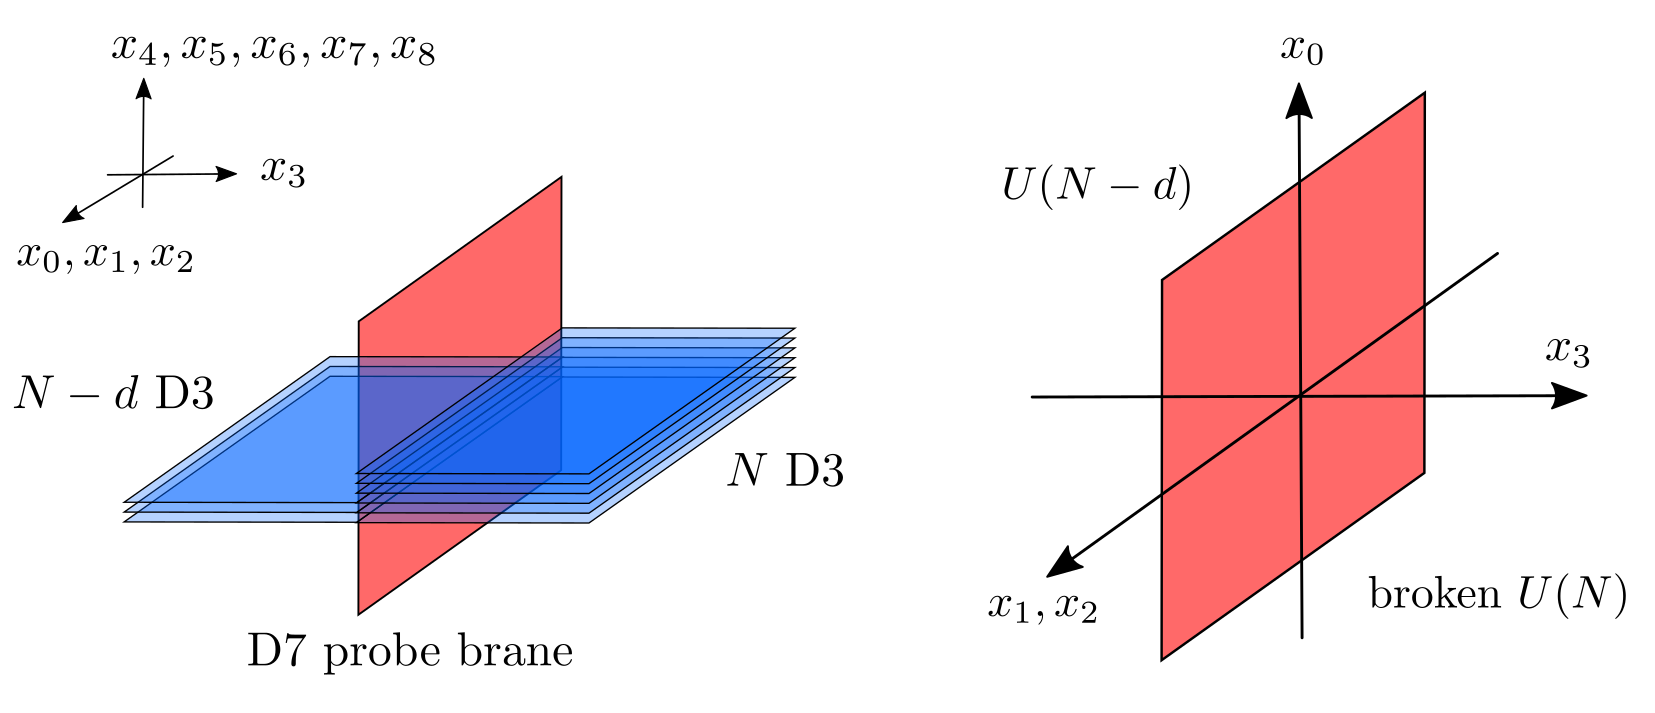
\includegraphics[width=1.0\textwidth]{../pics/brane_vs_field_setup_new.png}
%
\caption[Brane configuration vs. field theory configuration]{The brane configuration in string theory on the left vs. the dual field theory configuration, with different gauge groups on each side of the defect at $x_3=0$, on the right. This figure has been recreated from \cite{One-point functions in D3-D7}.}
%
\label{fig:probe-brane-setup}
%
\end{center}
%
\end{figure}
%
%

\subsection{Symmetries of the dCFTs}
Let us at this point briefly discuss what symmetries of the $\mathcal{N}=4$ SYM field theories survive the introduction of a defect in spacetime. First of all, the presence of the defect quite obviously break translation invariance in the direction perpendicular to itself. Also, the local $U(N - k_1 k_2)$ gauge symmetry in the $x_3 < 0$ region is trivially intact, since we have only zero vevs on this side of the defect. More interesting is the non-zero vevs in the $x_3 > 0$ region, which result from the classical scalar field solutions (\ref{cl solution 1}) and (\ref{cl solution 2}). These vevs partially break both the local $U(N)$ gauge group and the global $PSU(2,2|4)$ super conformal symmetry group of $4D$ $\mathcal{N} = 4$ SYM theory. From the forms of the scalar field solutions, we see that the global $PSU(2,2|4)$ symmetry reduces to the following.
%
%
\begin{equation}
PSU(2,2|4) \to SO(3,2) \times
\begin{cases}
	SO(3) \times SO(3) \\
	SO(5) \\
\end{cases}
\end{equation}
%
%
Where clearly, the upper case corresponds to (\ref{cl solution 1}) vevs, and the lower case corresponds to (\ref{cl solution 2}) vevs. We see that super symmetry is completely broken in these setups, which will become apparent when we look at the mass spectrum of the fields in subsection \ref{diag mass matrix}. The remaining spacetime symmetry is constituted by the Poincar\'e transformations parallel to the defect: $SO(2,1)$, and dilatations of spacetime: $SO(1,1)$, together with special conformal transformations that complete $SO(3,2)$. As already mentioned, the $U(N)$ gauge group is also partially broken by the non zero vevs, and is reduced to the following.
%
%
\begin{equation}
U(N) \to
\begin{cases}
	U(N - k_1 k_2) \times U(1) \times U(1) \\
	U(N - d_n) \times U(1) \\
\end{cases}
\end{equation}
%
%
Where the upper and lower cases again correspond to $\mathfrak{so}(3) \times \mathfrak{so}(3)$ and $\mathfrak{so}(5)$ symmetric vevs respectively. This is easily seen, as only multiples of $\mathbb{1}_{k_1}$, $\mathbb{1}_{k_2}$ commutes with $t_i^{k_1}$, $t_i^{k_2}$ respectively. Similarly, only multiples of $\mathbb{1}_{d_n}$ commutes with $G_{i6}^{d_n}$. Thus, the scalar field solutions $\Phi_i$ commutes with matrices of the form: $U = e^{i \theta_1} \mathbb{1}_{k_1} \otimes e^{i \theta_2} \mathbb{1}_{k_2} \oplus U_{N - k_1 k_2}$, in the $\mathfrak{so}(3) \times \mathfrak{so}(3)$ case, and matrices of the form: $U = e^{i \theta} \mathbb{1}_{d_n} \oplus U_{N - d_n}$, in the $\mathfrak{so}(5)$ case. However, because the gauge group in the $x_3 < 0$ region is given by either $U(N - k_1 k_2)$ or $U(N - d_n)$, any gauge transformation in the $x_3 > 0$ region has to reduce to either $U(N - k_1 k_2)$ or $U(N - d_n)$ transformations at the boundary. This is only possible for the subset of unitary transformations above, for which $\theta_1 = 0$, $\theta_2 = 0$ for the $\mathfrak{so}(3) \times \mathfrak{so}(3)$ case, and $\theta = 0$ for the $\mathfrak{so}(5)$ case. Thus, the gauge group in both cases is further reduced, so that the gauge groups on both sides of the defect agrees.
%
%
\begin{equation}
U(N) \to
\begin{cases}
	U(N - k_1 k_2) \\
	U(N - d_n) \\
\end{cases}
\end{equation}
%
%

\subsection{The aim of the thesis}
The primary focus of this thesis will be to study different kinds of bulk-to-bulk two-point functions in $\mathcal{N} = 4$ defect conformal field theories, with vevs given by either (\ref{cl solution 1}) or (\ref{cl solution 2}). More precisely, we will be looking at two-point functions of various local scalar single-trace operators $\mathcal{O}_a(x)$ and $\mathcal{O}_b(y)$, where the indicies $a$, $b$ label operators of the form.
%
%
\begin{equation}
\mathcal{O}_{a,b}(x) = \Psi_{a,b}^{i_1 \ldots i_L} \tr[\boldsymbol{\phi}_{i_1}(x) \ldots \boldsymbol{\phi}_{i_L}(x)]
%
\quad , \quad
%
x_3,y_3 > 0
\end{equation}
%
%
One-point functions between certain operators of the above types, have already been studied in \cite{One-point functions in D3-D7} for the case of $\mathfrak{so}(3) \times \mathfrak{so}(3)$ symmetric vevs, and in \cite{One-point functions in D3-D7 SO(5)} for the case of $\mathfrak{so}(5)$ symmetric vevs. The techniques developed in \cite{One-point functions in D3-D7,One-point functions in D3-D7 SO(5)} will also be intrumental in computing two-point functions, and so will the ideas presented in \cite{Length L length 2 two-point functions D5-D3}. The structure of this thesis will be as follow. First, in section \ref{sec:dCFT}, we will go through the necessary steps to bring the theory to a form suitable for making perturbatively calculations, of which the biggest challenge is to diagonalize all the new quadratic terms in the Lagrangian. We then proceed, in section \ref{sec:CPO}, to pertubativly compute the leading order contributions to two-point functions of different scalar single-trace chiral primary operators. Lastly, in section \ref{sec:NPO}, we attempt to compute the leading order contribution to the two-point fuctions of a certain type of non-protected operators with definite conformal dimension at 1-loop level, and single-trace scalar operators of length two.

%\subsection{Residual symmetry}
%Representative expressions involving $\Phi_i$ after expansion of action. 
%%
%%
%\begin{equation}
%[\tilde{\phi}_i, \Phi_j]
%%
%\to
%%
%[U \tilde{\phi}_i U^\dagger, \Phi_j]
%%
%=
%%
%U [\tilde{\phi}_i , U^\dagger \Phi_j U] U^\dagger
%\end{equation}
%%
%%
%
%%
%%
%\begin{equation}
%[\Phi_i, \Phi_j]
%%
%\to
%%
%[\Phi_i, \Phi_j]
%%
%=
%%
%U [U^\dagger \Phi_i U , U^\dagger \Phi_j U] U^\dagger
%\end{equation}
%%
%%
%
%%
%%
%\begin{equation}
%D_\mu \Phi_i
%%
%=
%%
%\partial_\mu \Phi_i - i [A_\mu, \Phi_i]
%%
%\to
%%
%\partial_\mu \Phi_i - i [U A_\mu U^\dagger + i U \partial_\mu U^\dagger, \Phi_i]
%\end{equation}
%%
%%
%\begin{equation}
%=
%%
%U \partial_\mu (U^\dagger \Phi_i U) U^\dagger -i U [A_\mu, U^\dagger \Phi U] U^\dagger
%%
%=
%%
%U D_\mu (U^\dagger \Phi_i U) U^\dagger
%\end{equation}
%%
%%
%All is good, so long as:
%%
%%
%\begin{equation}
%U^\dagger \Phi_i U = \Phi_i
%%
%\quad \Rightarrow \quad
%%
%[\Phi_i, U] = 0
%\end{equation}
%%
%%

